%%%%%%%%%%%%%%%%%%%%%%%%%%%%%%%%%%%%%%%%%
% Short Sectioned Assignment
% LaTeX Template
% Version 1.0 (5/5/12)
%
% This template has been downloaded from:
% http://www.LaTeXTemplates.com
%
% Original author:
% Frits Wenneker (http://www.howtotex.com)
%
% License:
% CC BY-NC-SA 3.0 (http://creativecommons.org/licenses/by-nc-sa/3.0/)
%
%%%%%%%%%%%%%%%%%%%%%%%%%%%%%%%%%%%%%%%%%

%----------------------------------------------------------------------------------------
%	PACKAGES AND OTHER DOCUMENT CONFIGURATIONS
%----------------------------------------------------------------------------------------

\documentclass[a4paper,11pt]{scrartcl} % A4 paper and 11pt font size

\usepackage[T1]{fontenc} % Use 8-bit encoding that has 256 glyphs
\usepackage[utf8]{inputenc}
\usepackage{fourier} % Use the Adobe Utopia font for the document - comment this line to return to the LaTeX default
\usepackage[english]{babel} % English language/hyphenation
\usepackage{amsmath,amsfonts,amsthm} % Math packages

\usepackage{lipsum} % Used for inserting dummy 'Lorem ipsum' text into the template
\usepackage{graphicx}
\usepackage{sectsty} % Allows customizing section commands
\allsectionsfont{\centering \normalfont\scshape} % Make all sections centered, the default font and small caps

\usepackage{fancyhdr} % Custom headers and footers
\pagestyle{fancyplain} % Makes all pages in the document conform to the custom headers and footers
\fancyhead{} % No page header - if you want one, create it in the same way as the footers below
\fancyfoot[L]{} % Empty left footer
\fancyfoot[C]{} % Empty center footer
\fancyfoot[R]{\thepage} % Page numbering for right footer
\renewcommand{\headrulewidth}{0pt} % Remove header underlines
\renewcommand{\footrulewidth}{0pt} % Remove footer underlines
\setlength{\headheight}{13.6pt} % Customize the height of the header

\numberwithin{equation}{section} % Number equations within sections (i.e. 1.1, 1.2, 2.1, 2.2 instead of 1, 2, 3, 4)
\numberwithin{figure}{section} % Number figures within sections (i.e. 1.1, 1.2, 2.1, 2.2 instead of 1, 2, 3, 4)
\numberwithin{table}{section} % Number tables within sections (i.e. 1.1, 1.2, 2.1, 2.2 instead of 1, 2, 3, 4)

\setlength\parindent{0pt} % Removes all indentation from paragraphs - comment this line for an assignment with lots of text

%----------------------------------------------------------------------------------------
%	TITLE SECTION
%----------------------------------------------------------------------------------------

\newcommand{\horrule}[1]{\rule{\linewidth}{#1}} % Create horizontal rule command with 1 argument of height

\title{	
\normalfont \normalsize 
\textsc{Universidade de Brasília} \\ [25pt] % Your university, school and/or department name(s)
\horrule{0.5pt} \\[0.4cm] % Thin top horizontal rule
\huge Configurando a Ponte Rolante \\ % The assignment title
\horrule{2pt} \\[0.5cm] % Thick bottom horizontal rule
}

\author{Ataias Pereira Reis \\ Emanuel Pereira Barroso Neto} % Your name

\date{\normalsize\today} % Today's date or a custom date

\begin{document}

\maketitle % Print the title

%----------------------------------------------------------------------------------------
%	PROBLEM 1
%----------------------------------------------------------------------------------------

\section{Conexões Importantes}
\paragraph{} O presente documento tem por objetivo ser um guia prático para a configuração do sistema da ponte rolante a ser utilizado na validação experimental do controle de \textit{risers} em malha fechada.

%------------------------------------------------

\subsection{Componentes}

%------------------------------------------------

\subsubsection{Controlador Lógico-Programável}
\begin{figure}[!ht]
  \centering
    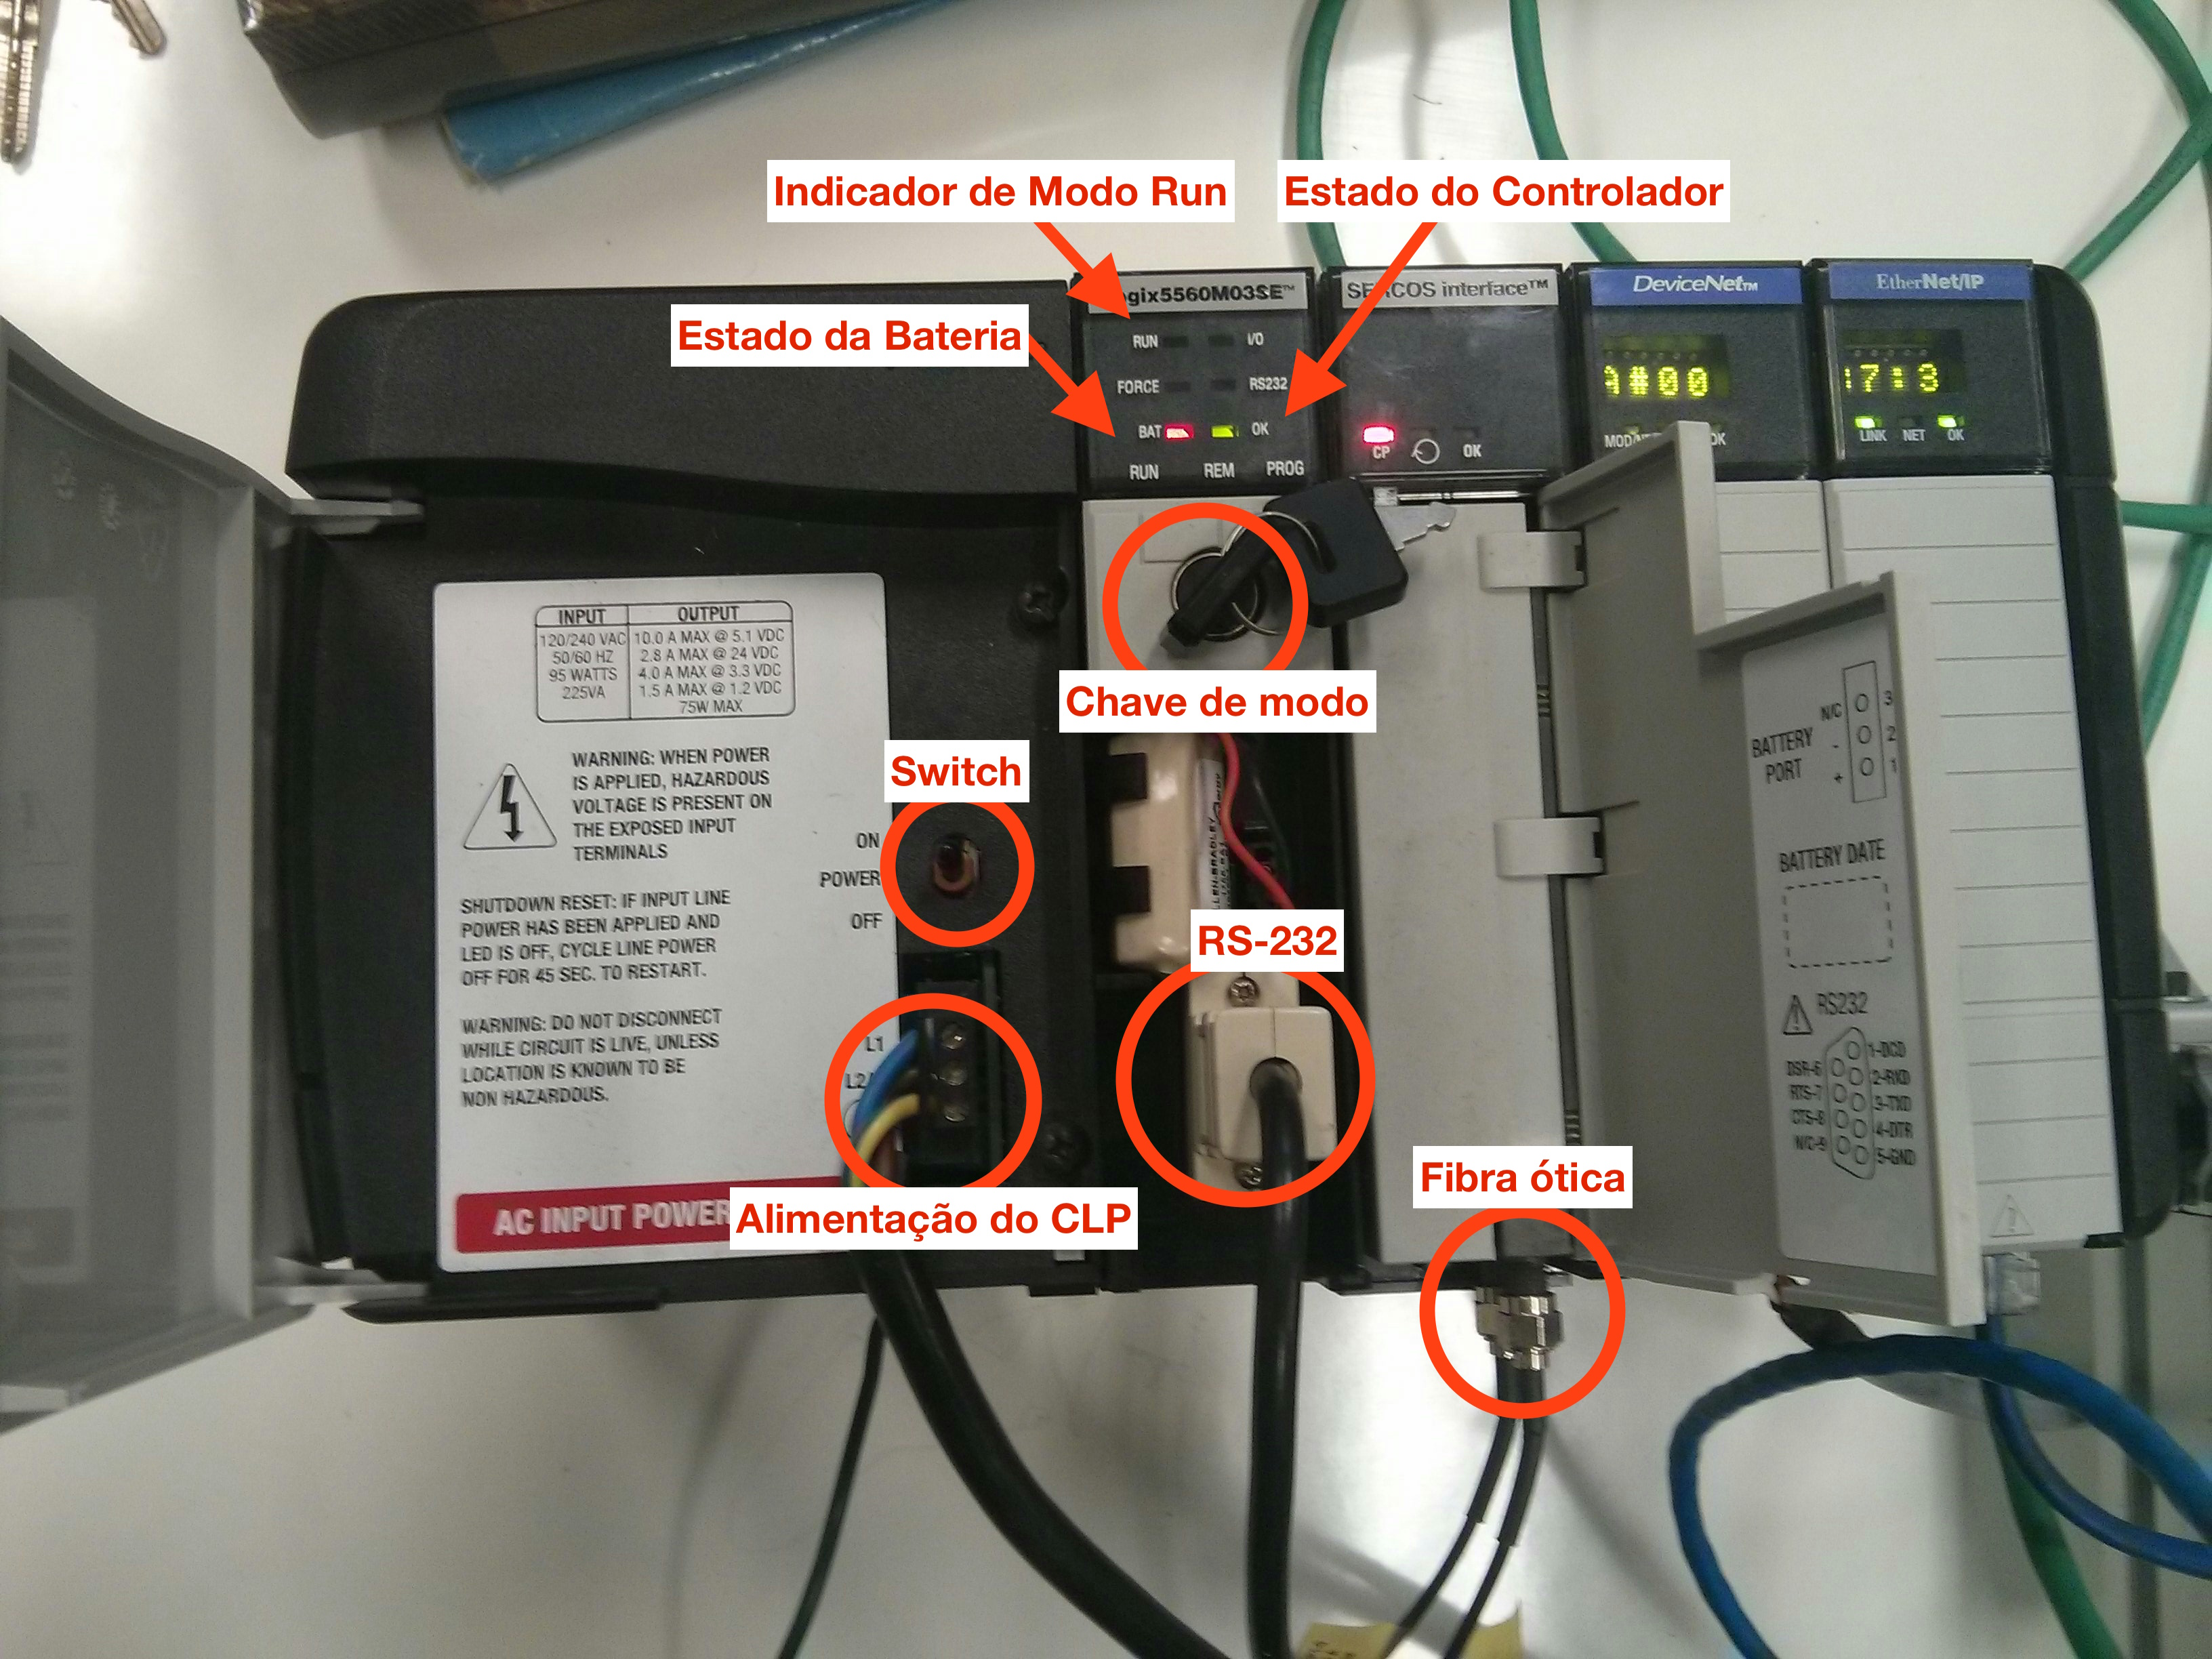
\includegraphics[width=1\textwidth]{figures/hardware/CLP.jpg}
    \caption{CLP com identificação de elementos\label{CLPcomentado}}
\end{figure}

\paragraph{} O controlador lógico-programável (CLP - ver Figura \ref{CLPcomentado}) é a espinha dorsal da bancada. Ele é responsável por executar os comandos de controle vindos do computador sobre todos os elementos que estão conectados a ele.
\paragraph{} O CLP utilizado é fabricado pela \textit{Allen Bradley}, modelo Logix5560M03SE. Tal modelo possui memória lógica e de dados de 750 KiB, e memória de \textit{I/O} de 494 KiB. Há quatro módulos no \textit{chassis} do controlador:
\begin{itemize}
  \item O próprio controlador;
  \item \textit{SERCOS Interface};
  \item DeviceNET;
  \item EtherNet/IP.
\end{itemize}
\paragraph{} Além dos módulos, o controlador ainda possui um \textit{switch} liga/desliga presente no \textit{chassis}. No módulo Logix, há uma chave responsável por alterar o modo de funcionamento do mesmo. As posições possíveis dessa chave são:
\begin{itemize}
  \item RUN;
  \item REM;
  \item PROG;
\end{itemize}
\paragraph{} Na prática, o modo REM se divide em dois modos: REM RUN e REM PROG. A maneira de se diferenciar os dois é observar, no módulo Logix, o estado do LED indicador de modo RUN quando a chave estiver na posição REM.
\paragraph{} No modo RUN, o controlador apenas roda o programa presente em sua memória; não há qualquer comunicação remota. No modo PROG, o controlador não roda nenhum programa; ele apenas pode receber um novo código. Nos modos REM, há a comunicação com o computador, permitindo verificar valores de variáveis de interesse e alterar, se necessário, o programa a ser rodado pelo controlador. O programa presente no controlador, em modo REM, só roda o código se estiver no modo REM RUN; se for necessário atualizar o programa, o modo deve ser o REM PROG.

\subsubsection{DeviceNET}
\paragraph{} O DeviceNET é a rede responsável por estabelecer a conexão do controlador lógico-programável com os sensores indutivos. A rede é alimentada com 24 Volts externa, pois o módulo DeviceNET não fornece tal alimentação.
\paragraph{} A rede DeviceNET também está conectada a um módulo de saídas, o \textit{CompactBlock I/O}. Esse bloco, na presente configuração, apenas transmite a alimentação da fonte de 24 V para os sensores e o módulo DeviceNET. A alimentação da rede também foi conectada à alimentação da câmera.

\subsubsection{Sensores Indutivos}
\paragraph{} Os sensores indutivos são elementos detectores de presença, particularmente de objetos metálicos. Eles funcionam através da variação de campo magnético ocasionada pela presença do objeto a ser identificado. Tal variação de campo magnético provoca uma variação de corrente dentro do sensor, alterando seu estado.
\paragraph{} Na presente bancada, há 6 sensores indutivos da família 871TM, fabricados pela \textit{Allen Bradley}. Eles são alimentados com tensão de 24 V, que está dentro dos limites padrão. São sensores feitos de aço, adaptados a ambientes industriais.

\subsection{Cuidados com as conexões e com o controlador}
\paragraph{} Para que o sistema funcione corretamente, alguns cuidados devem ser tomados:
\begin{enumerate}
  \item A rede DeviceNET deve ser alimentada corretamente; caso contrário, o módulo DeviceNET emitirá uma mensagem de erro \textit{``No Network Power''}; caso essa mensagem seja mostrada, os sensores indutivos também não estarão alimentados, e não funcionarão.
  \item O \textit{switch} liga/desliga do controlador é protegido por uma tampa. É recomendável que, com o controlador em operação, que esta tampa esteja fechada.
  \item Atentar para o estado do disjuntor industrial; ele deve estar ligado para que o motor funcione.
  \item Não retirar a chave de modo do controlador; sem ela, pode ser impossível carregar um novo programa para o controlador ou mesmo rodar um programa já carregado.
\end{enumerate}

%----------------------------------------------------------------------------------------
%	PROBLEM 2
%----------------------------------------------------------------------------------------

\section{Lists}

%------------------------------------------------

\subsection{Example of list (3*itemize)}
\begin{itemize}
	\item First item in a list 
		\begin{itemize}
		\item First item in a list 
			\begin{itemize}
			\item First item in a list 
			\item Second item in a list 
			\end{itemize}
		\item Second item in a list 
		\end{itemize}
	\item Second item in a list 
\end{itemize}

%------------------------------------------------

\subsection{Example of list (enumerate)}
\begin{enumerate}
\item First item in a list 
\item Second item in a list 
\item Third item in a list
\end{enumerate}

%----------------------------------------------------------------------------------------

\end{document}
